%----------------------------------------------------------------------------------------
%	DATA ACQUISITION AND PREPARATIONS
%----------------------------------------------------------------------------------------

\section{Data acquisition and organization}

The value and purpose of a study project does not only lie in the implementation and realization of a long-term scientific study - in our case, computer vision-based label prediction to improve an agricultural sorting machine - but also in learning to organize, schedule, and distribute tasks for a larger team over the period of one year. \\
 \\
To accomplish the objective of the project, a working structure had to be established. The project members had to learn each other's strengths and weaknesses to form a robust and efficient unit. Self-organization and team building became key to the success of the project. Thus, the secondary focus of the report lies on the management of the study group. \\
The process of team building and structuring is captured in the first half of this chapter. A timeline of the different working stages can be traced in a roadmap created at the start and updated at the end of the year. It reveals how well the team succeeded in predicting the duration of the various tasks. \\
Further, the communication between the members is addressed which includes regular meetings, agreements on different issues, or the working platforms that were used. Additionally, the teamwork is evaluated which comprises task distribution, the democratic working structure, and the (structural) integrity of the team. \\
After the organizational part of the project, the second half of this chapter is concerned with the collection of the data and the literature research. The sorting machine is described as well as the process of saving and retrieving the recorded images. It is followed by a summary of the literature which was thought to be relevant to our topic regarding the visual detection of agricultural products or images with low variance with machine learning approaches. There was no specific paper, however, which could be used as a basis for our project. \\
\\
The first section of this chapter, 2.1 Timetable (roadmap) of the project, gives an overview of the time management of the study group. \\
It is followed by the chapter 2.2 Organization of the study group, in which communication and teamwork are assessed. \\
In 2.3 Data collection, the acquisition of the data from the sorting machine is described in more detail. \\
The last section, 2.4 Literature research, presents the collected literature concerning our issue.


\subsection{Timetable (roadmap) of the project}

At the beginning of the project, a roadmap was created to structure the year into different working stages as well as to have an overview of the tasks and problems that needed to be addressed. Near the end of the year, this map was evaluated and updated to mirror the actual time spent at each project stage and to check how accurately the project had been planned from the start. If there were great discrepancies between estimation and reality, the map helped to acknowledge the wrong judgement of time and which working stages had taken longer than others. \\
\\
The following timetables in Figure~\ref{fig:Timetable} give a broad outline of the major stages of the project. In the left figure, it was estimated how much time for a specific phase is needed, whereas in the right figure the time spent for the stage is given. Both figures are structured to display the year in a circle, starting in April of 2019, and running clockwise through the year until April 2020. The months are represented by the inner circle while the outer circle marks the different working stages. \\
The project comprised four to five major stages. The following stage descriptions are shortened for the purpose of simplicity. A more detailed representation of the single tasks attributed to each stage can be found in the ensuing roadmaps in Fig.~\ref{fig:RoadmapPlanned} and Fig.~\ref{fig:RoadmapActual}. The project started with the Data Collection and the Organization of the study project. During the first stage, the images were recorded with the sorting machine, while the major planning and research for the project took place. In the second phase, most of the Preprocessing happened, that is, preparing and labelling the image data. This phase is split into two phases for the right figure displaying the actual time, ‘Preprocessing’ and ‘Labelling’. The classification stage includes the time spent on the machine learning approaches which were implemented and trained on the asparagus data. In the last stage, the approaches were evaluated and their results were compared. It is noteworthy that the different stages overlapped to a certain degree, because minor tasks of a previous stage were still in progress while tasks from the subsequent stage had already started. For the purpose of this figure the start and end time is displayed as a hard boundary. \\
\\

\begin{figure}[h]
	\centering
	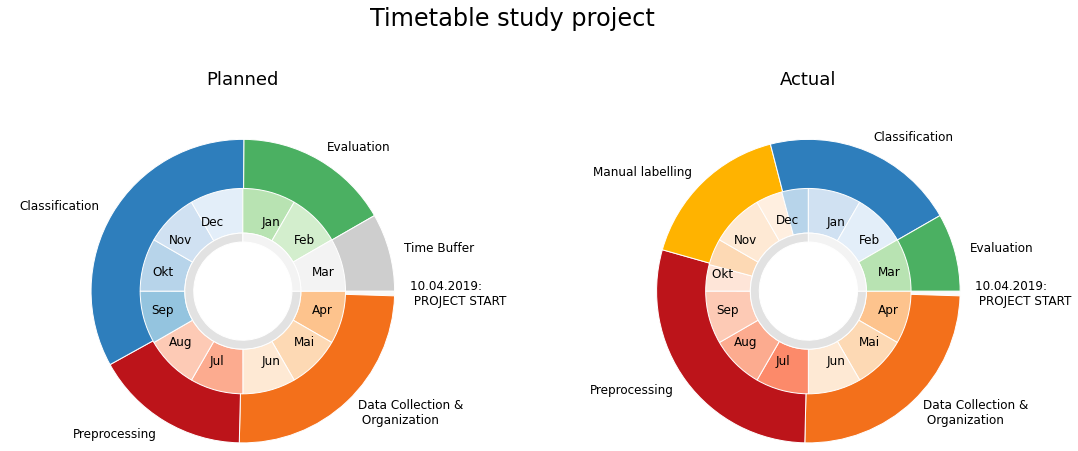
\includegraphics[scale=0.4]{Figures/chapter02/fig_timetable}
	\decoRule
	\caption[Timetable of the project]{On the left side is a timetable with the estimated time of the study project during the year from April 2019 to April 2020. To the right, the timetable displays how the time was spent.}
	\label{fig:Timetable}
\end{figure}

When comparing both figures, some distinctions can be recognized. The figure to the left shows that - while it was noted that the Preprocessing step of labelling the data would take some time - it was not estimated to take longer than until the end of August. Compared to the Preprocessing step in the right figure, it is observed that the phase continued until October. Furthermore, the time for labelling a sufficient amount of images was underestimated. In the right figure, the labelling process received its own stage to highlight the fact that it demanded much more effort and time compared to the initial estimation.
This exchange required that the time buffer and parts of the time calculated for the later stages of classification and evaluation had to compensate for the time loss.
The time difference can best be seen when comparing the respective colours (that is, the brighter colours of red, orange and yellow to the darker colours of blue and green). While the main focus of this project was supposed to be the application of different machine learning techniques to classify the data, the data generation and preprocessing posed to be the most time-consuming stages. \\
As a result, both timetables differ in that the year was more optimistically planned than realized. A major factor was the lack of experience of the participants concerning not only the conduction of a larger project with many co-workers but also the general implementation of the preprocessing stage for machine learning classification. Another factor influencing the shifted timeline was the working structure of the team. It was re-evaluated during October to better fit the needs of the group members and avoid distributing so-called ‘bottleneck’ tasks (that is, tasks that are decisive for the continuation of the next steps) to single members only. All in all, a valuable lesson learned during the project was to not underestimate a preprocessing phase. \\

\begin{figure}[h]
	\centering
	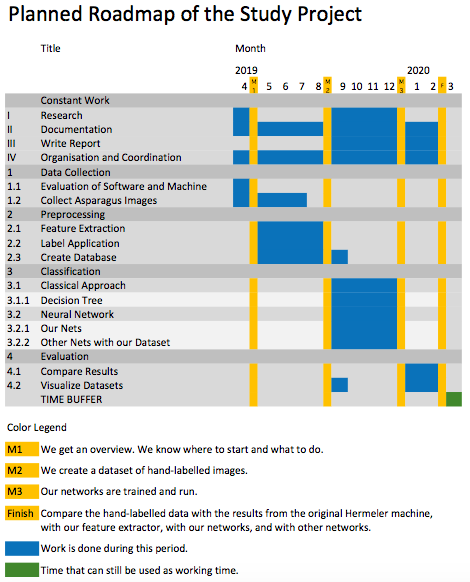
\includegraphics[scale=0.5]{Figures/chapter02/roadmap_planned}
	\decoRule
	\caption[Planned Roadmap]{The figure shows the planned roadmap of the study project. It reveals how the time needed for each task was estimated in the beginning of the project.}
	\label{fig:RoadmapPlanned}
\end{figure}

\begin{figure}[h]
	\centering
	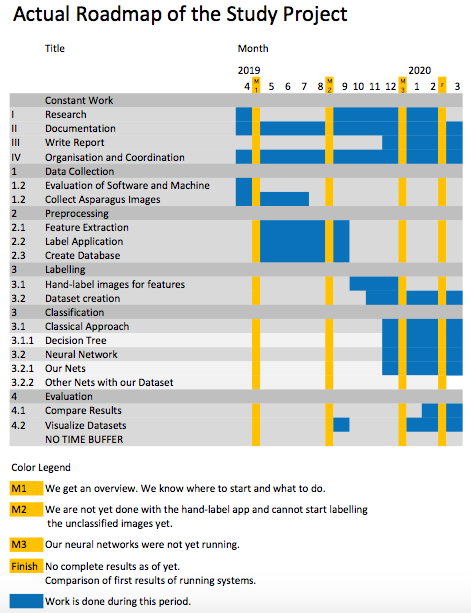
\includegraphics[scale=0.5]{Figures/chapter02/roadmap_actual}
	\decoRule
	\caption[Actual Roadmap]{A roadmap that shows how the time was spent.}
	\label{fig:RoadmapActual}
\end{figure}
\\
In Figure~\ref{fig:RoadmapPlanned} and Figure~\ref{fig:RoadmapActual}, the stage specific tasks can be seen in more detail. Again, both figures display the estimated time and the actual time, respectively. The headlines serve as the division into the major stages except for the first heading, ‘Constant Work’, which shows the tasks that demanded continuous attention and effort throughout the year. The duration of tasks is represented in blue, while the yellow lines mark milestones that are explained in their legends. \\
\\
Comparing both roadmaps, the shift of focus is seen more clearly and can be associated with the duration of single tasks. Especially the prominent drift of the classification stage mirrors the fact that the time estimation is worth improving. The roadmap helped to better assess the time needed for task completion.
In the following chapter, the management of the work distribution and the communication are taken into focus.


\subsection{Organisation of the study group}

In this chapter, we will describe how we have organized ourselves to work together on the project. For this we will elaborate on the tools we used for communication and organization as well as on the structure of our group work and our teamwork in general.


\subsubsection{Communication}

Our main way of communication were frequent meetings in which we discussed our process work period and distributed tasks for the next one. In addition to those meetings, we used different platforms, which worked with varying degrees of success. After a presentation about possible strategies of cooperation, we initially decided to use Asana, GitHub and Telegram to facilitate the communication outside of our meetings. The different means of communication will be described and evaluated in the following abstract. \\
\\
Regular meetings have been the most helpful in organizing our project. During the meetings, which usually lingered for one or two hours, there was a discussion leader and a protocol writer. The protocols were saved for review in our GitHub project. The meetings were characterized by long discussions about the best approach for the following steps and the possibilities to tackle the next challenge. Our supervisors were almost always present at the meetings, they brought in their expertise and gave us the opportunity to ask concrete questions. During the first half of the project, tasks were always distributed at the end of each meeting and in the next meeting the progress of the work was discussed. The communication was changed in the second half of the project,  where we started to use a schedule that described the different tasks and deadlines in detail, and to gather for co-working. The organizational meetings were continued and used to discuss the current status with Ulf and Axel. Everyone reported about his area of responsibility. This helped us to spend less time discussing and debating and more time working on our tasks.
Telegram is a cloud-based instant messaging service for the use on smartphones, tablets and computers. Since the first meeting, we had a constant conversation in a group chat on Telegram, in which we arranged us for the weekly meetings, planned hand-overs of keys/transponders for the room or informed each other about the status of the project. The group chat also created space for mutual motivation when needed. The majority of important information was exchanged via telegram. \\
Asana is used to distribute tasks and to communicate projects successfully. Many integrations of other applications, such as Slack, can help to achieve this. We used a board view where we listed tasks in different sections. But this function alone did not help us much in our project. The tasks were easier to distribute in direct consultation at physical meetings and demonstrated or discussed after completion. So it happened that Asana was not used enough to be helpful. If we had relied on communication with Slack or other agreed services or applications, it might have made more sense, but asana alone was proven to be inefficient in our use case. \\
GitHub is a web-based popular platform using a version control system using Git that helps developers store and manage their code, and track and control changes to their project. During the project, we learned how to use it. Initially, a presentation was given by Katharina on how to use Git, because there are a few rules to follow to keep it straightforward. Git allowed us to work from anywhere, which was very helpful for us. We also automatically created a documentation with Sphinx.


\subsubsection{Teamwork}

This subchapter outlines the team forming, the team members and the cooperation in our study project. It starts by introducing the team members and their previous experiences. This is followed by a description of the practical aspects of teamwork, the work structure, and the distribution of project-relevant tasks. \\
\\
First, the team members and their respective backgrounds are illustrated before delving into further work-related task distributions. \\
The project was an initiative of one of the students and, hence, a large part of the project members are friends that were inspired by her ideas. Other students joined the project after its public announcement to complete the team. Thus, the group consisted of members with varying degrees of knowledge about each other, which had an influence on the dynamics of the teamwork. The team was initially made up by Malin Spaniol, Maren Born, Katharina Groß, Josefine Zerbe, Michael Gerstenberger, Richard Ruppel, Sophia Schulze-Weddige, Luana Vaduva, Thomas Klein and Subir Das. None of the members had yet worked together as such on a project of this scope. During the course of the project, three members left the team for various reasons. Thomas left in July due to a change in his study program. This was an unfortunate occurrence because he posed a valuable source of knowledge in the field of computer vision. Further, Luana and Subir left in October to pursue different study projects. \\
\\
By the start of the project, all except two of the members were in their master’s degree in Cognitive Science at the University of Osnabrück. The members brought a wide variety of backgrounds into the team through different bachelor programs or different majors in the broader field of cognitive science.
In the beginning of the project, the team members had little to no experience in the application of computer vision or neural networks. The motivation of most students was to pursue new and interesting tasks in these fields. Four students had a theoretical background in computer vision, six students had gained some experience with neural networks through the course ‘ANN with Tensorflow’, taught at the University of Osnabrück, while some had also taken machine learning classes during their study program. None of the members had prior knowledge about project management or task organization on a broader level. Git was previously only used by three students so far, but none of them were experts on its usage. Further, no participant had any experience with the Grid system of the IKW, not to mention running jobs on different machines. \\
Thus, the project started with 10 members, where each of the participants brought a different level of experience in the most relevant fields of machine learning, that is computer vision and neural networks, into the team.\\
\\
After introducing the team members and their backgrounds, this section continues with elaborating the structural organization of the team and the work distribution.
As none of the members had any previous experience with team formation, in the beginning, the team lacked some structure and a clear distribution of single roles inside the team. One reason for this was the harmonious atmosphere between the single members. Many of the team members had a friendly relationship already from the start of the project. Also, further tasks at the beginning, like the trips to the asparagus farm, strengthened the team spirit and the social interactions positively. So we started with a very dynamic structuring of tasks by making every decision democratically. As described in more detail in the next chapter, we first used the joint meetings to distribute the tasks. As an example, we had to prepare a schedule for organizing the data collection and already started with preprocessing tasks. These two main activities were mostly done in smaller teams of two to three people. Rather few tasks were done alone. In our meetings, we often formulated possible next tasks, even for the distant future, but as the project progressed we did not assign them to a specific person or working group. \\
In August, we restructured our own organization. On the one hand, this was due to the fact that the tasks changed and thus a new structure was more appropriate. On the other hand, also the weaknesses of the individual team members were a reason for the restructuring. Some team members had less programming experience than others and therefore had difficulties realizing certain tasks at the same time and with the same precision than others. Even if they had good ideas in terms of concept, it was not possible for them to implement these ideas quickly enough so that they could be included into the project. In addition, the democratical self-organization and difference in programming expertise led to a distortion in the time management of the group and some tasks were not finished in time (with other tasks). To integrate more of the strengths that the single team members brought and to tackle the issue of time management, it was decided to write a roadmap that distributed the work more appropriately, gave an overview of the tasks that still had to be done and how much time was left to do them.
Further, common working hours on campus were introduced as well as a division of responsibilities (work-related and related to the supervision of tasks). The common working hours ensured that questions and decisions that arose could be discussed directly. This was especially helpful when different tasks overlapped and required communication and agreement.
The supervision of the work was divided into manager roles, which means that the work was split into different main fields where each member was responsible for managing their assigned area, distributing tasks and keeping an overview of the relevant work inside their working field. Furthermore, one knew who to turn to for questions and when in need of discussion or feedback. The meetings became more effective due to the new structure, and there was less discussion concerning task distribution. As we distributed roles, we were also more responsive to the strengths and weaknesses of the group members. \\
Therefore one can say that the team structure and distribution of work changed over the course of the project. The strengths of single members were used more efficiently and the supervision of working areas led to a more structured supervision and manageable task distribution. \\
\\
In summary, we can say that we have not only learned new scientific skills and techniques of data acquisition, preparation, and analysis but also gained valuable new insights into the organization of a large project with many members. We  understood how to organize ourselves more successfully and purposefully. First and foremost, we learned that this includes excellent communication. The whole team agrees that we would structure the next project in the same way as we did in the second half from the beginning on. Communication is important, but it was discovered that there is a right way to balance the amount and effectiveness of communication. Not everyone has to discuss or listen to all the details in every area, often it suffices when all team members have a broad overview.
Additionally, it turned out to be helpful when, one or two members exchange some of the task-related work in favour of more management-related work. This helps to gain a better team structure, time management, and, in the end, make the team work more effectively and efficiently towards its goal. \\
Specifically, the experience of two different working structures gave us the ability to better judge how good teamwork is achieved, how each member can better include themselves into the team, and what each member can improve for future teamwork. As the main intention of the study project was understood as a learning unit, we wanted to seek out tasks that we are motivated to do and that bring us new experiences and skills, and not just practice what we already know. \\
\\
\\
In the course of the project and to sum up the focus of this chapter, namely the organisation of our study group, it can be said that we had a harmonious team with two different working structures, one cultivated at the start of the project and the other one at the end of the project, respectively, which happened due to the tasks amount and the optimisation of our teamwork. We have all learned that teamwork is not a trivial issue, even for members who already know each other well.


\subsection{Data collection}

TODO: How we collected the data and what the data looked like. \\

INTRODUCTION
\begin{itemize}
\item Driving to asparagus farm "Gut Holsterfeld"
\item First look at the data.
\end{itemize}

MAIN
\begin{itemize}
\item First problem: no labelled data.
\item The asparagus sorting machine
\begin{itemize}
\item How is the data recorded?
\item How are labels calculated? Could we use them?
\end{itemize}
\item Second problem: image saving stop after 1000 images.
\item First solution: Teamviewer sessions.
\end{itemize}

SECOND SOLUTION: File moving service \\
\\
The requirements for the software are described below. Because of the problems described, a solution was requested that runs in the background and does not disturb the workflow during the sorting process. The operating system on which the sorting machine runs is Windows. Consequently, after some internet research on background processes and programs, the decision was made to use a service. Windows was used, therefore, the development was done with the DOTNET framework in the programming language C#. As discovered during the internet research, the package provided is called "Topshelf" (\url{https://github.com/Topshelf/Topshelf}). Topshelf is a service hosting framework for building Windows services using .NET. This makes it possible to develop a console application in the development phase, compile it as a service and install it later via the console. Previously, it was not possible to debug services. The function of the service is based on the FileSystemWatcher object (\url{https://docs.microsoft.com/en-us/dotnet/api/system.io.filesystemwatcher?view=netframework-4.8}) from the System.IO namespace. In the main program a list of files in the source folder is kept. Files older than one hour are moved to the target folder on the external drive. The selected files are moved by a function that is called, when an event is triggered. The event is triggered by the FileSystemWatcher after subscribing to different flags. After a short time the service was adjusted. Then, we introduced the described hourly waiting time, because the program of the sorting machine itself still accesses the images indefinitely.

\subsection{Literature research}

TODO: Previous literature research concerning food classification.

\begin{itemize}
\item Searching for background literature close to our project, e.g. automatic CV-based sorting of other food products.
\item Researching semi-supervised and unsupervised learning approaches.
\item Re-reading on potential ANN structures that we could use for sorting.
\item What was the result?
\item Could we rely on a certain paper/process? Did it work?
\end{itemize}


